% This file was created with tikzplotlib v0.10.1.
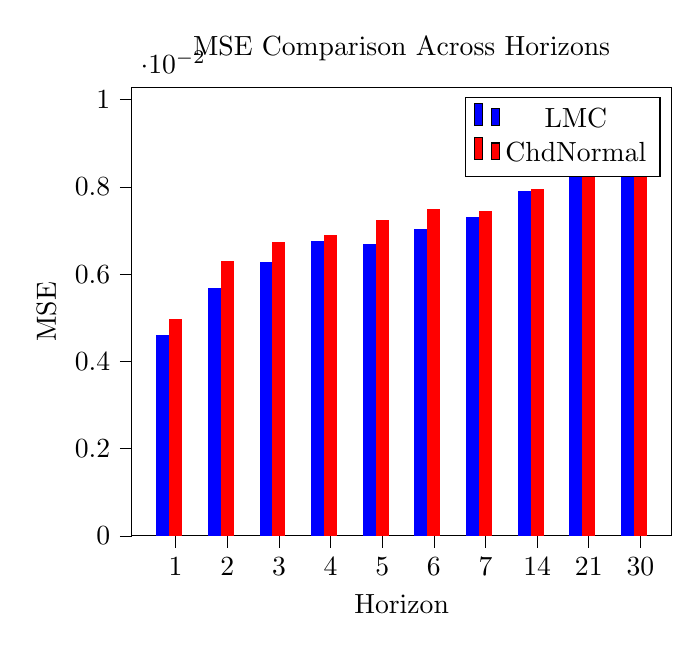
\begin{tikzpicture}

\definecolor{darkgray176}{RGB}{176,176,176}

\begin{axis}[
tick align=outside,
tick pos=left,
title={MSE Comparison Across Horizons},
x grid style={darkgray176},
xlabel={Horizon},
xmin=-0.85, xmax=9.6,
xtick style={color=black},
xtick={0,1,2,3,4,5,6,7,8,9},
xticklabels={1,2,3,4,5,6,7,14,21,30},
y grid style={darkgray176},
ylabel={MSE},
ymin=0, ymax=0.0102792028206475,
ytick style={color=black}
]
\draw[draw=none,fill=blue] (axis cs:-0.375,0) rectangle (axis cs:-0.125,0.00460906041761763);
\addlegendimage{ybar,ybar legend,draw=none,fill=blue}
\addlegendentry{LMC}

\draw[draw=none,fill=blue] (axis cs:0.625,0) rectangle (axis cs:0.875,0.00568826781759324);
\draw[draw=none,fill=blue] (axis cs:1.625,0) rectangle (axis cs:1.875,0.00627408472704168);
\draw[draw=none,fill=blue] (axis cs:2.625,0) rectangle (axis cs:2.875,0.00676607178363412);
\draw[draw=none,fill=blue] (axis cs:3.625,0) rectangle (axis cs:3.875,0.00670202694845332);
\draw[draw=none,fill=blue] (axis cs:4.625,0) rectangle (axis cs:4.875,0.00703125204354492);
\draw[draw=none,fill=blue] (axis cs:5.625,0) rectangle (axis cs:5.875,0.00730232933822083);
\draw[draw=none,fill=blue] (axis cs:6.625,0) rectangle (axis cs:6.875,0.00790971205412464);
\draw[draw=none,fill=blue] (axis cs:7.625,0) rectangle (axis cs:7.875,0.00847351603799065);
\draw[draw=none,fill=blue] (axis cs:8.625,0) rectangle (axis cs:8.875,0.0090488782525174);
\draw[draw=none,fill=red] (axis cs:-0.125,0) rectangle (axis cs:0.125,0.00497566504068967);
\addlegendimage{ybar,ybar legend,draw=none,fill=red}
\addlegendentry{ChdNormal}

\draw[draw=none,fill=red] (axis cs:0.875,0) rectangle (axis cs:1.125,0.00630389905185345);
\draw[draw=none,fill=red] (axis cs:1.875,0) rectangle (axis cs:2.125,0.00674500810433079);
\draw[draw=none,fill=red] (axis cs:2.875,0) rectangle (axis cs:3.125,0.00689939848777731);
\draw[draw=none,fill=red] (axis cs:3.875,0) rectangle (axis cs:4.125,0.0072501422445004);
\draw[draw=none,fill=red] (axis cs:4.875,0) rectangle (axis cs:5.125,0.007496271073825);
\draw[draw=none,fill=red] (axis cs:5.875,0) rectangle (axis cs:6.125,0.00745837907829539);
\draw[draw=none,fill=red] (axis cs:6.875,0) rectangle (axis cs:7.125,0.00794303745744196);
\draw[draw=none,fill=red] (axis cs:7.875,0) rectangle (axis cs:8.125,0.00848497737877072);
\draw[draw=none,fill=red] (axis cs:8.875,0) rectangle (axis cs:9.125,0.00934472983695226);
\end{axis}

\end{tikzpicture}
